% =======================================================================
%
%                                SETUP
%
% =======================================================================

\documentclass[12pt, oneside]{article}
\usepackage[utf8]{inputenc}
\usepackage[IL2]{fontenc}
\usepackage{hyperref} 
\usepackage[czech, english]{babel}
\usepackage{graphicx}
\graphicspath{ {./static/} }
\usepackage{geometry}
\geometry{
	left=4cm,
	top=4cm,
	right=4cm,
	bottom=4cm
}

\pagenumbering{gobble}

% =======================================================================
%
%                                CONTENT
%
% =======================================================================

\begin{document}

\thispagestyle{empty}
\begin{center}
	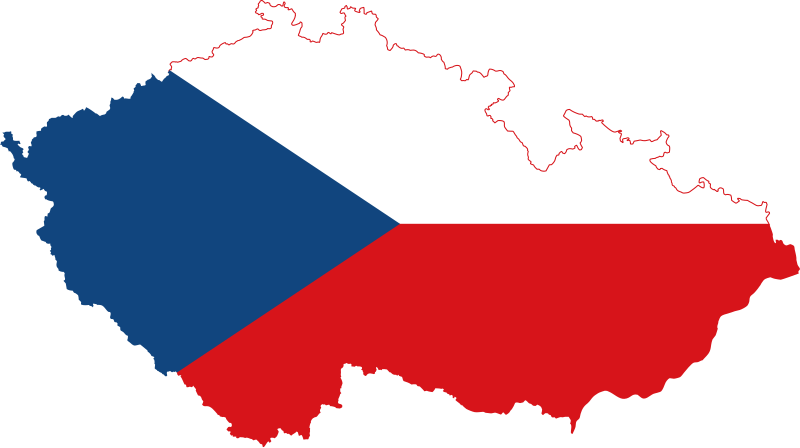
\includegraphics[width=10cm]{map.png}
	
  \vspace*{4em}

  \rule{\linewidth}{0.5mm}
  \vspace*{1em}
  
  {\LARGE Czechia – a thorough Geoguessr guide} \\ [1cm]
	\textbf{\Large Marek Smolík}
  \\ \texttt{spalovac\_mrtvol@discord}
  \\ \texttt{\href{https://github.com/dynamo58}{GitHub}}
  \\ \texttt{\href{https://www.twitch.tv/bigladmush22}{Twitch profile}}
  \\ \texttt{\href{https://www.geoguessr.com/user/5ee78ead03f80c500c7cba22}{Geoguessr profile}}
  \vspace*{1em}
  \\ Last edited:\ \today
  \\ Version:\ \texttt{0.0}


  \vspace*{1em}
  \rule{\linewidth}{0.5mm}
\end{center}

\newpage

\tableofcontents

\newpage

\begin{abstract}
Czechia or the Czech republic is a country notoriously difficult. For one thing it is very difficult to region-guess and at times also to distinguish from some of the surrounding countries. This document tries to outline all of the possible metas and actual geography knowledge there is to be obtain in order to guess this country accuretly and be able to make informed region-guesses within the country itself.
\end{abstract}

\clearpage

\pagenumbering{arabic}
\setcounter{page}{1}

\section{Introduction}

\subsection{About the author}

My name is Marek Smolík and I am a fellow Geoguessr player. I have lived in Czechia my whole life and played Czechia extensively on Geoguessr, speedrunning it among other gamemodes. As such I have accumulated knowledge that is not necessarily well-known. I have no intention in trying to gatekeep this information... the complete opposite... actually.

\subsection{Contribution}

All types of contribution to this doc are welcome. Contribution may include a suggestion, a dispute of correctness about something included, etc. If you wish to contribute to this document you can do so through any of the on the title page. Preferred way is opening an issue on \href{https://github.com/dynamo58/geoguessr-czechia-guide}{this doc's GitHub page} or outright opening a pull request. But getting hang of me on any of the other platforms is also fine. All the contribees will be included in the \hyperref[sec:ack]{Acknowledgements section} if they choose so.

\newpage
\section{Recognizing the country}

\newpage
\section{Region-guessing the country}

\newpage
\section{Acknowledgements}
\label{sec:ack}

\subsection{External graphics}

This document's graphics are incorporated partially from external sources. Special thanks goes to them, wherever they may be. The following is their list:

\begin{itemize}
  \item Title page Czechia map\cite{gr1}
\end{itemize}

\subsection{Contribees}


% =======================================================================
%
%                                BIBLIOGRAPHY
%
% =======================================================================

\begin{thebibliography}{e}
\bibitem{gr1}
Flag-map of the Czech Republic. "Stasyan117." 2015. \textit{Wikimedia.org}. Wikimedia Commons. Web. 16 September 2024.


\end{thebibliography}

\end{document}
